\documentclass[tikz,border=2pt]{standalone}
\usepackage{amsmath,amssymb}
\usepackage{xcolor}
\usetikzlibrary{arrows.meta,positioning,calc,fit,backgrounds,shapes.misc}

% ------- styles & macros -------
\tikzset{
  line/.style={-Stealth, line width=0.6pt},
  mc/.style={draw, rectangle, minimum width=6mm, minimum height=6mm, inner sep=0pt},
  bus/.style={draw, rectangle, inner sep=3mm},
  sum/.style={draw, circle, inner sep=0pt, minimum size=9pt},
  lab/.style={fill=white, inner sep=1pt}
}
\newcommand{\vL}{V_{\mathcal L}}
\newcommand{\vH}{V_{\mathcal H}}
\newcommand{\vhatL}{\hat{v}_{\mathcal L}}
\newcommand{\vhatH}{\hat{v}_{\mathcal H}}
\newcommand{\ihat}{\hat{\imath}}

\begin{document}
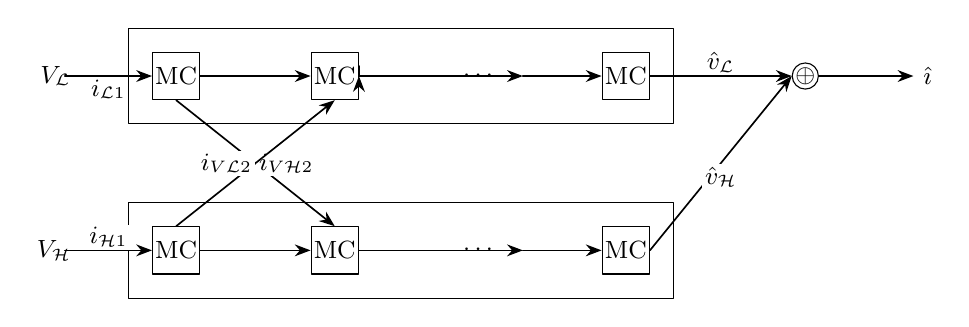
\begin{tikzpicture}[font=\small, >=Stealth, node distance=14mm, line cap=round, line join=round]

  % ---- top row MCs ----
  \node[mc] (t1) {MC};
  \node[mc, right=14mm of t1] (t2) {MC};
  \node[right=12mm of t2] (tdots) {$\cdots$};
  \node[mc, right=12mm of tdots] (t4) {MC};

  % ---- bottom row MCs ----
  \node[mc, below=16mm of t1] (b1) {MC};
  \node[mc, right=14mm of b1] (b2) {MC};
  \node[right=12mm of b2] (bdots) {$\cdots$};
  \node[mc, right=12mm of bdots] (b4) {MC};

  % ---- containers (fit) with left labels ----
  \node[bus, fit=(t1)(t2)(tdots)(t4), label={[xshift=-6mm]left:$\vL$}] (busL) {};
  \node[bus, fit=(b1)(b2)(bdots)(b4), label={[xshift=-6mm]left:$\vH$}] (busH) {};

  % ---- left inputs to first MCs ----
  \coordinate (L_in) at ($(busL.west)+(-8mm,0)$);
  \coordinate (H_in) at ($(busH.west)+(-8mm,0)$);
  \draw[line] (L_in) -- (t1.west)
      node[midway, below, lab] {$i_{\mathcal L 1}$};
  \draw[line] (H_in) -- (b1.west)
      node[midway, above, lab] {$i_{\mathcal H 1}$};

  % ---- forward links within rows ----
  \draw[line] (t1.east) -- (t2.west);
  \draw[line] (b1.east) -- (b2.west);
  % 通过省略号的连线(分两段以避开“⋯”节点)
  \draw[line] (t2.east) -- ($(tdots.east)+(2mm,0)$);
  \draw[line] ($(bdots.east)+(2mm,0)$) -- (b4.west);
  \draw[line] (t2.east) ++(0,0) -- ++(0,0); % 占位,易于对齐
  \draw[line] (b2.east) -- ($(bdots.east)+(2mm,0)$);
  \draw[line] ($(tdots.east)+(2mm,0)$) -- (t4.west);

  % ---- cross links (diagonals) ----
  \draw[line] (t1.south) -- (b2.north)
      node[midway, right, lab] {$i_{V\mathcal{H}2}$};
  \draw[line] (b1.north) -- (t2.south)
      node[midway, left, lab] {$i_{V\mathcal{L}2}$};

  % ---- outputs to adder ----
  \node[sum, right=18mm of t4] (adder) {$\oplus$};
  \draw[line] (t4.east) -- (adder.west)
      node[midway, above, lab] {$\vhatL$};
  \draw[line] (b4.east) -- (adder.west)
      node[midway, below, lab] {$\vhatH$};
  \draw[line] (adder.east) -- ++(12mm,0) node[right] {$\ihat$};

\end{tikzpicture}
\end{document}